\begin{exercise}

Analysiere den Beweis des Satzes über die offene Abbildung und zeige folgende
allgemeinere Variante: \\

Sei $X$ ein Banachraum, $Y$ ein normierter Raum und sei $A: X \rightarrow Y$ stetig
und linear und $A(X)$ sei von 2. Kategorie (für die Terminologie siehe Bemerkung
4.1.4 im Skriptum) in $Y$.
Dann folgt:

\begin{enumerate}[label = (\roman*)]
  \item $A$ ist offen.
  \item $A(X) = Y$.
  \item $Y$ ist Banachraum.
\end{enumerate}

\end{exercise}

\begin{solution}

\phantom{}

\begin{enumerate}[label = (\roman*)]

  \item
  Jedes Element von $X$ liegt in einer hinreichend aufgeblasenen Kugel.

  \begin{align*}
    X = \bigcup_{k \in \N} U_k^X(0)
  \end{align*}

  Diese Darstellung setzen wir in $A$ ein.

  \begin{align*}
    A(X)
    =
    A \pbraces
    {
      \bigcup_{k \in \N}
      U_k^X(0)
    }
    =
    \bigcup_{k \in \N}
    A(U_k^X(0))
  \end{align*}

  Die Voraussetzung, $A(X)$ sei von 2. Kategorie besagt, dass sich $A(X)$ nicht als abzählbare Vereinigung von \blockquote{nirgends dichten} Mengen darstellen lässt.
  Also, soll eine der Mengen, in der oberen Vereinigung, nicht \blockquote{nirgends dicht} sein.
  D.h. $\Exists k \in \N:$

  \begin{align*}
    W := \overline{A(U_k^X(0))}^\circ \neq \emptyset.
  \end{align*}

  $W$ ist offen und nichtleer und $+$ stetig.
  Daraus folgt, dass $W - W$ eine offene Nullumgebung ist. \\

  Aufgrund der Stetigkeit on $+$, in Form von $+(\overline{A \times B}) \subseteq \overline{+(A \times B)}$, folgt

  \begin{align*}
    W - W
    \subseteq
    \overline{A(U_k^X(0))} + \overline{A(U_k^X(0))}
    \subseteq
    \overline{A(U_k^X(0)) + A(U_k^X(0))}
    =
    \overline{A(U_k^X(0) + U_k^X(0))}
    =
    \overline{A(U_{2k}^X(0))}.
  \end{align*}

  Sei $\epsilon > 0$, sodass

  \begin{align*}
    U_{\epsilon}^Y(0)
    \subseteq
    W - W
    \subseteq
    \overline{A(U_{2k}^X(0))}.
  \end{align*}

  Schließlich, müssen wir unsere Abbildung $A$ noch skalieren.

  \begin{align*}
    B := \frac{2k}{\epsilon} A
  \end{align*}

  Aufgrund der Stetigkeit von $\cdot$, folgt

  \begin{align*}
    U_1^Y(0)
    =
    \frac{1}{\epsilon} U_{\epsilon}^Y(0)
    \subseteq
    \frac{1}{\epsilon} \overline{A(U_{2k}^X(0))}
    \subseteq
    \overline{A(U_{\frac{2k}{\epsilon}}^X(0))}
    = \overline{\frac{\epsilon}{2k}B(U_{\frac{2k}{\epsilon}}^X(0))}
    =
    \overline{B(U_{1}^X(0))}.
  \end{align*}

  Lemma 4.3.3 liefert uns dann sogar diese Inklusion, ohne Abschluss.

  \begin{align*}
    U_1^Y(0) \subseteq B(U_{1}^X(0))
  \end{align*}

  Laut Lemma 4.3.2 ist $B$ damit eine offene Abbildung. \\

  Sei nun aber $O \subseteq X$ eine beliebige offene Menge.

  \begin{align*}
    A(O)
    =
    \frac{\epsilon}{2k}B(O)
  \end{align*}

  $A(O)$ ist offen, da $B(O)$ offen und die Skalarmultiplikation ein Homöomorphismus ist.
  Somit ist auch $A$ eine offene Abbildung.

  \item
  Wir wissen also, dass $A(X)$ offen, und, aufgrund der Linearität von $A$, ein linearer Teilraum von $Y$ ist.
  Aus Aufgabe 3/2 wissen wir, dass jeder echter linearer Teilraum von $Y$ keinen inneren Punkt hat und
  daher nicht offen sein kann.
  Deswegen muss $A(X) = Y$.

  \item
  $A: X \to Y$ ist ein Homomorphismus.
  Sei $N := \ker(A)$.
  Der Homomorphiesatz für Vektorräume besagt, es gibt genau einen Homomorphismus $\varphi: X/N \to Y: A = \varphi \circ \kappa$.
  Dabei, ist $\kappa: X \rightarrow X/N: x \mapsto [x]_{\sim_N}$ die kanonische Einbettung.

  \begin{center}
  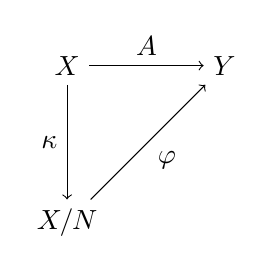
\begin{tikzpicture}[auto]
      \node (X) at (0,0) {$X$};
      \node (X/N) at (0,-2) {$X/N$};
      \node (Y) at (2,0) {$Y$};
      \draw[->] (X) to node  {$A$} (Y);
      \draw[->] (X) to node [swap]  {$\kappa$} (X/N);
      \draw[->] (X/N) to node [swap] {$\ExistsOnlyOne \varphi$} (Y);
  \end{tikzpicture} \\
  \end{center}

  $(X, \norm{\cdot})$ ist ein Banachraum.
  Laut Proposition 2.4.9, ist $(X/N, \norm[X/N]{\cdot}$ ebenfalls Einer.
  $A$ ist surjektiv, also $\varphi$ sogar ein Isomorphismus. \\

  Wir zeigen schließlich noch, dass $\varphi$ ebenfalls eine offene Abbildung ist.
  Sei dazu $O \in \mathcal{T}_{\norm[X/N]{\cdot}}$.
  Dies ist genau dann der Fall, wenn $[O]_{\sim_N}$ offen in $X$ ist.

  \begin{align*}
    \varphi(O)
    & =
    \Bbraces
    {
      \varphi([x]_{\sim_N}):
      [x]_{\sim_N} \in O
    }
    =
    \Bbraces
    {
      (\varphi \circ \kappa)(x):
      [x]_{\sim_N} \in O
    }
    =
    \Bbraces
    {
      A(x):
      [x]_{\sim_N} \in O
    } \\
    & =
    \bigcup_{[x]_{\sim_N} \in O}
    A(\Bbraces{x})
    =
    \bigcup_{[x]_{\sim_N} \in O}
    A([x]_{\sim_N})
    =
    A \Bigg
    (
      \underbrace
      {
        \bigcup_{[x]_{\sim_N} \in O}
        [x]_{\sim_N}
      }_{
        [O]_{\sim_N}
      }
    \Bigg)
    =
    A([O]_{\sim_N})
  \end{align*}

  \begin{align*}
    A ~\text{offen}
    \implies
    \pbraces
    {
      \Forall O \in \mathcal{T}_{\norm[X/N]{\cdot}}:
      A([O]_{\sim_N}) ~\text{offen}
    }
    \implies
    \pbraces
    {
      \Forall O \in \mathcal{T}_{\norm[X/N]{\cdot}}:
      \varphi(O) ~\text{offen}
    }
    \implies
    \varphi ~\text{offen}
  \end{align*}

  Daraus folgt, dass $\varphi^{-1}$ stetig ist und somit (weil linear) beschränkt.
  Laut Bemerkung 4.3.5, ist das äquivalent dazu, dass $\Exists a > 0: \Forall [x]_{\sim_N} \in X/N:$

  \begin{align*}
    a \norm{[x]_{\sim_N}}
    \leq
    \norm{\varphi([x]_{\sim_N})}.
  \end{align*}

  Damit, sind alle Voraussetzungen für Lemma 4.3.6 erfüllt.
  Angewendet auf $\varphi$ und $X/N$, folgt schlussendlich, dass $Y$ ein Banachraum ist.

\end{enumerate}

\end{solution}
